\documentclass{article}

\usepackage{a4wide}
\usepackage[utf8]{inputenc}
\usepackage[T1]{fontenc}
\usepackage[french]{babel}
\usepackage[babel=true]{csquotes} 
\usepackage{graphicx}
\graphicspath{{Images/}}
\usepackage{color}
\usepackage{hyperref}
\hypersetup{colorlinks,linkcolor=,urlcolor=blue}

\usepackage{amsmath}
\usepackage{amssymb}
\usepackage{mathrsfs}


\usepackage{graphicx}



\title{Rapport - Programmation concurrente}
\author{Elisabeth ZETTOR, L3 informatique}
\date{\today}

\begin{document}

\maketitle % pour écrire le titre


%% Le résumé:
\begin{abstract}
  Dans ce rapport, je vais vous montrer ce que nous avons pu voir en programmation concurrente cette année, ainsi que les exercices que nous avons effectués, et notamment quelques points que j'ai pu trouver difficiles ou importants.
\end{abstract}

\section{Introduction}
\label{section : intro}

\begin{center}

\end{center}
En programmation concurrente, nous avons pu apprendre à programmer des threads, notamment en Python et en Java, dont l'intérêt était de pouvoir décomposer un programme en tâches pouvant s'effectuer simultanément. Le but des exercices que nous avons effectués était donc de nous familiariser avec cette notion, et de pouvoir utiliser les threads de manière correcte (i.e. les arrêter convenablement (thread démon ou interrompu), utiliser des verrous...).

\section{Exercices}
\label{section : exercices}

\subsection{Première partie des exercices : Bases}
\label{section : base}


\subsubsection{Threads simples}
\label{section : threadsimples}

Dans cette partie, nous devions écrire un programme qui devait lancer deux threads en fonction des paramètres que nous entrions dans la console. Cet exercice, comme son nom l'indique~(\ref{section : threadsimples}), nous a permis de créer nos premiers threads. Nous avons pu notamment voir qu'il était nécessaire de mettre les instructions propres à un thread dans une fonction \begin{it}run()\end{it} qui possède un "bloc spécial" afin d'éviter les exceptions et de générer des erreurs : 
\begin{verbatim}
public void run() {
		try {
			//instructions
		} catch (InterruptedException e) { }
}
\end{verbatim}

Et, afin de démarrer le thread, il fallait le lancer avec la méthode \begin{it}start()\end{it}.

Voici l'exercice en java:
\begin{center}
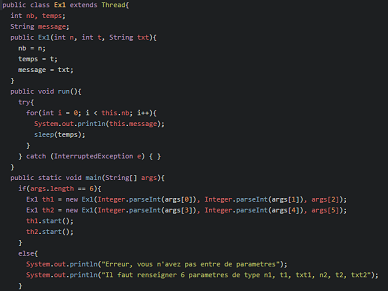
\includegraphics{ex1_1.png}
\end{center}

\subsubsection{Interruption de threads}
\label{section : interruptionthread}

Ici, le but était de mettre en lumière le principe d'interruption, qui permet d'interrompre un thread prématurément depuis un autre thread, étant donné qu'un thread s'achève normalement naturellement à la fin de l'exécution de sa méthode \begin{it}run()\end{it}.
Ici, il fallait interrompre manuellement les threads grâce à la méthode \begin{it}interrupt()\end{it} et la méthode \begin{it}interrupted()\end{it} qui permet de savoir si oui ou non le thread a été interrompu.

Ainsi, dans la fonction \begin{it}run()\end{it}, on rajoute une boucle while, afin d'arrêter le thread lorsqu'on celui est interrompu (déclenché lorsqu'on appuie sur une touche du clavier). Ce qui donne :
\begin{verbatim}
public void run() {
		try {
				while(!interrupted()){
						//instructions
				}
		} catch (InterruptedException e) { }
}
\end{verbatim} 



Voici un morceau de code en Python:
\begin{center}
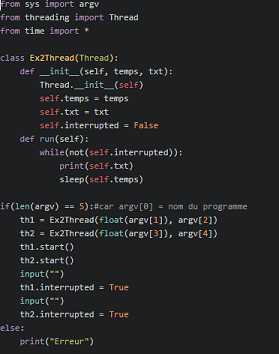
\includegraphics{ex1_2py.png}
\end{center}


\subsubsection{Threads démons}
\label{section : threaddemon}

Enfin, nous avons montré l'intérêt des threads démons. Rendre un thread démon nous permet de ne pas avoir à l'arrêter manuellement, à l'inverse de l'interruption. Ainsi: \begin{quote} \begin{it}"Si tous les threads sont des démons, alors ces derniers sont arrêtés brutalement et le programme se termine."\end{it} \end{quote}
Cependant, lorsqu'on utilise des threads démons, il faut absolument utiliser la méthode \begin{it}setDaemon()\end{it} avant d'utiliser la méthode \begin{it}start()\end{it}, sinon on obtient des erreurs.

Voici une portion de code en Java:
\begin{center}
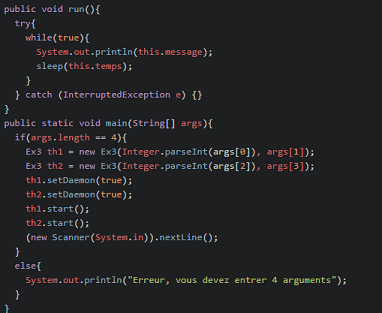
\includegraphics{ex1_3.png}
\end{center}

\subsection{Deuxième partie des exercices : Coordination de threads - Producteurs et consommateurs}
\label{section : deuxiemepartie}

Dans cette partie, c'est la notion d'attente et de notification qui est démontrée. Grâce à cette méthode, nous pouvons éviter les problèmes d'interblocages et de famine et donc nous pouvons mettre en place le principe d'exclusion mutuelle. Autrement dit: \begin{quote}\begin{it}"L'exclusion mutuelle est la propriété qu'à tout instant deux tâches ne peuvent se trouver en section critique, i.e. au plus une tâche est en train d'exécuter une instruction de la section critique."\end{it}\end{quote}
Cependant, le procédé est différent selon le langage utilisé. Ainsi, en Python, on va utiliser les verrous, avec la classe \begin{it}RLock()\end{it} et utilisation de l'instruction \begin{it}with\end{it} ou bien, on va utiliser la classe \begin{it}Condition()\end{it} qui dispose des méthodes \begin{it}wait()\end{it} et \begin{it}notifyAll()\end{it}, ce qui est assez similaire à Java dans ce cas-ci.
En Java, on va pouvoir utiliser les méthodes synchronisées, combinées avec les méthodes \begin{it}wait()\end{it} et \begin{it}notityAll()\end{it}.

\subsubsection{Affichage d'un nombre et de son carré}
\label{section : carre}

Le but de cet exercice était, comme son nom l'indique, d'afficher un nombre et son carré. Nous avons donc crée une classe Producteur (un thread) qui prenait un nombre, l'incrémentait et calculait son carré, et une autre classe Consommateur (thread). Le rôle de cette classe était d'afficher le nombre et son carré. Cependant, si l'on lance les deux threads sans utiliser d'attente et de notifications, on peut afficher le même nombre et le même carré plusieurs fois ou manquer un nombre et son carré, d'où l'utilisation des méthodes \begin{it}wait()\end{it} et \begin{it}notifyAll()\end{it}.

Voici une démonstration du programme dans la console :
\begin{center}
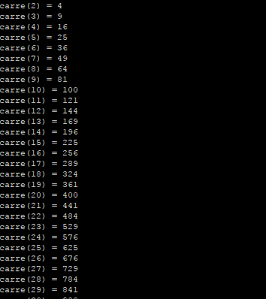
\includegraphics{ex2_1.png}
\end{center}

\subsubsection{Compte en banque}
\label{section : banque}

Ici, même principe que pour la section \ref{section : carre}, mais avec un compte en banque, où l'on dépose et où l'on retire aléatoirement une somme, uniquement si c'est possible. Seulement, ici, on lance plusieurs threads consommateurs.

Voici une démonstration de l'exercice dans la console :
\begin{center}
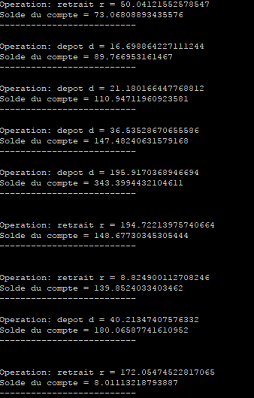
\includegraphics{ex2_2.png}
\end{center}

\subsubsection{File d'entiers}
\label{section : file}

Ici, même principe, avec une file d'entiers. On crée trois classes:
\begin{itemize}
\item File: qui comporte plusieurs méthodes: une pour ajouter un entier si la file n'est pas pleine, une autre pour en retirer si la file n'est pas vide, et une autre pour afficher;
\item Producteur : elle se charge d'ajouter les entiers à la file;
\item Consommateur : elle se charge de retirer des entiers.
\end{itemize}

\subsection{Troisième partie des exercices : Threads et interfaces graphiques avec Swing et Tkinter}
\label{section : interfaces}

\subsubsection{Producteurs et consommateurs}
\label{section : prodcons}

Le but ici était de reprendre les exercices précédents et de les présenter avec une interface graphique en Python et en Java, en utilisant Swing~\cite{swingDoc} et Tkinter~\cite{tkinterDoc} (python). 
Ainsi, si nous reprenons l'exercice des files~\ref{section : file}, il fallait uniquement modifier les fonctions d'affichage, afin de pouvoir visualiser le texte dans une fenêtre et associer à un bouton start l'action de lancer les threads, avec en paramètre des threads, les labels qui sont modifiés dans la fenêtre.

Voici une démonstration de l'exercice des files avec interface graphique avec tkinter :
\begin{center}
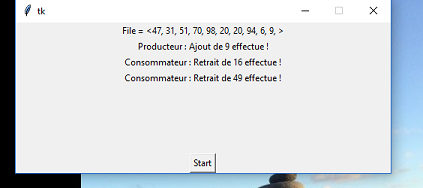
\includegraphics{ex3_1.png}
\end{center}

\subsubsection{Balles en mouvement}
\label{section : balles}

Cet exercice est une mise en pratique de tout ce que nous avons vu plus haut. Ainsi pour mener à bien ce projet (en Java), nous avons dû créer 6 classes:
\begin{itemize}
\item Affichage : c'est dans cette classe que nous affichons les balles et qu'on incrémente le score lorsqu'une collision se produit;
\item Balle : c'est dans cette classe qu'on crée notre objet Balle, qui a des coordonnées de position, une couleur générée aléatoirement;
\item Balles : dans cette classe, on crée une liste d'objets Balle, avec une méthode ajouteBalle() afin d'ajouter des éléments lorsqu'on appuie sur le bouton "+";
\item Fenetre : c'est la classe qui permet de mettre en place notre interface, avec les labels correspondants au score, au temps, les boutons "start" qui permet d'enclencher le mouvement des balles, et qui se transforme en bouton stop pour mettre sur pause, le bouton "+" qui permet de rajouter des balles, et le bouton "-" qui permet d'en retirer;
\item Mouvement : la classe qui permet de mettre en mouvement les balles et faire en sorte qu'elles ricochent sur les bords;
\item Timer : la classe qui permet de lancer le timer.
\end{itemize}




\section{Conlusion}

Ce cours était bien utile, notamment en ce qui concerne la création d'interfaces graphiques, pour éviter que le thread principal qui gère l'interface ne soit bloqué en essayant d'effectuer plusieurs tâces à la fois.


%%% La bibliographie:
\bibliographystyle{plain}
\bibliography{ma_biblio.bib}

\end{document}
